% Modelo de Dissertação em Latex para o PPG em Engenharia Elétrica - Sistemas Eletrônicos da UERJ
% Este modelo foi adaptado da versão disponibilizada no site da Engenharia Elétrica da UERJ
% http://www.pel.uerj.br/publico/Modelo_LaTeX_Dissertacao_UERJ.rar
% http://www.pel.uerj.br/defesas/
%
% 
%
% 
%
% 
% Atualizações:
% Felipe M. - 20/06/2012
% Fernando Lima - 15/07/2015
%





\documentclass[a4paper,12pt,oneside,openany]{uerj}

\usepackage[english,brazil]{babel}
%\usepackage[latin1]{inputenc}
\usepackage[utf8]{inputenc}
\usepackage{enumerate}
\usepackage{cite}
\usepackage{epsf,epsfig,./packages/psfig}
\usepackage{./packages/pagina}
\usepackage{indentfirst}
\usepackage{theorem}
\usepackage{fancyhdr}
\usepackage{setspace}
\usepackage{boxedminipage}
\usepackage{float}
\usepackage{makeidx}
\usepackage{amsmath}
\usepackage[hidelinks]{hyperref}




%%%%%% Definições %%%%%%%
\newtheorem{deff}{Definição}[section]
\numberwithin{equation}{chapter}

\theoremstyle{plain}

\bibliographystyle{./bib/abnt-num}


%%%%% DOC %%%%%%%%%%%%


\makeindex


\begin{document}

\hypersetup{
    colorlinks,
    citecolor=black,
    filecolor=black,
    linkcolor=black,
    urlcolor=black,
    linktoc=all
}

\thispagestyle{empty}\begin{titlepage}
\begin{center}

	\vspace{-0.5cm}

  \begin{figure}[hbt!]
		\begin{flushleft}
		   
\includegraphics[width=3.44cm,height=3.17cm]{./01_Pre_textuais/figures/logo_uerj_pb.png}
		\end{flushleft}
	\end{figure}
	\vspace{-4cm}

  \hspace{2cm}\large{\textbf{Universidade do Estado do Rio de Janeiro}}\\
  \hspace{2cm}\large{Centro de Tecnologia e Ciências}\\
  \hspace{2cm}\large{Faculdade de Engenharia}\\

  \hspace{2cm}\large{}\\
  \hspace{2cm}\large{}\\
  \hspace{2cm}\large{}\\
  \hspace{2cm}\large{}\\

  \par
  \large{Nome do Aluno}

  \hspace{2cm}\large{}\\
  \hspace{2cm}\large{}\\
  \hspace{2cm}\large{}\\
  \hspace{2cm}\large{}\\


  \par
  \large\textbf{Título do Trabalho}


  \par\vfill
  Rio de Janeiro\\2012

\end{center}
\end{titlepage}
\pagebreak\thispagestyle{empty}\begin{center}

Nome do Aluno

% \vfill
\vspace{2cm}

\textbf{Título do Trabalho}

\vspace{1.0cm}

\begin{figure}[hbt!]
\begin{center}

\includegraphics[width=10.48cm,height=10.8cm]{./01_Pre_textuais/figures/logo_uerj_gnd_pb.png}
\end{center}
\end{figure}

\vspace{-9cm}
\begin{flushright}
\parbox{8cm}{
\singlespacing{Dissertação apresentada, como requisito\linebreak parcial para obtenção do título de Mestre em Ciências, ao Programa de Pós-Graduação em Engenharia Mecânica, da Universidade do Estado do Rio de Janeiro. Área de\linebreak concentração: Fenômenos de Transporte}.
}
\end{flushright}

\vspace{4.0cm}

Orientador: Prof. Dr. Nome do Professor\\

\par\vfill
%\vspace{2cm}

Rio de Janeiro\\2012

\end{center}
\pagebreak\thispagestyle{empty}% Depois de preparar seu trabalho, você deverá enviá-lo para a Biblioteca CTC/B para avaliação do formato e elaboração da Ficha catalográfica.
% Com a ficha pronta (fornecida pela Biblioteca), você poderá alterar este trecho do trabalho em definitivo.
%
% Para este processo, enviei a dissertação em PDF para o email: ctcb.uerj.bdtd@gmail.com (Tratei de todos os detlahes com a Sra. Márcia)
% Qualquer dúvida, veja os contatos da Biblioteca no site da Rede Sirius: http://www.rsirius.uerj.br/
% 


\begin{titlepage}
	\begin{center}
\vfill
\singlespacing
	\vspace*{95mm}
	{CATALOGAÇÃO NA FONTE\\ \vspace{1.5mm}
	UERJ\,/\,REDE SIRIUS\,/\,BIBLIOTECA CTC/B}\\
	\vspace{1.5mm}
	\begin{boxedminipage}{140mm}
	\begin{minipage}{5mm}
		\vspace{-84mm}
		S237
	\end{minipage}
	\hfill
	\raisebox{8.5mm}{
	\begin{minipage}[top]{115mm}
		\vspace*{5mm}

		Sobrenome, Nome do Autor\\
		\phantom{XX}Título do trabalho\,/\,Nome completo do autor. -- 2012.\\
		\phantom{XX}105\,f.\\
		\phantom{XX}\\
		\phantom{XX}Orientadores: Nome do orientador1;\\
\hspace*{5mm}
 Nome do orientador1.\\
       		\phantom{XX}Dissertação(Mestrado) -- Universidade do Estado do Rio de Janeiro, Faculdade de Engenharia.\\
		\phantom{XX}\\
		\phantom{XX} Texto a ser informado pela biblioteca
	\end{minipage}}
	\vspace*{5mm}
	\begin{flushright}
	 CDU~621:528.8
	\end{flushright}
    \vspace{1mm}
	\end{boxedminipage}\\
	\end{center}
%
	Autorizo, apenas para fins acadêmicos e científicos, a reprodução total ou parcial desta dissertação, desde que citada a fonte.\\
	\noindent
	\begin{tabular}{ccc}
	\phantom{XXXXXXXXXXXXXXXXXXXXXXXXXXXXXX}&	 \phantom{XX}	&	\phantom{XXXXXXXXXXXXXXXX}	\\
	\phantom{XXXXXXXXXXXXXXXXXXXXXXXXXXXXXX}&	 \phantom{XX}	&	\phantom{XXXXXXXXXXXXXXXX}	\\
	\cline{1-1}\cline{3-3}
	Assinatura &		&	Data
	\end{tabular}
\end{titlepage} 
\pagebreak\thispagestyle{empty}\addtocounter{page}{+1}
\begin{center}

Nome do Aluno

\vspace{1cm}

\textbf{Título do Trabalho}

\end{center}

\vspace{.4cm}

\begin{flushright}
\parbox{8cm}{
\singlespacing{Dissertação apresentada, como requisito\linebreak parcial para obtenção do título de Mestre em Ciências, ao Programa de Pós-Graduação em Engenharia Mecânica, da Universidade do Estado do Rio de Janeiro. Área de\linebreak concentração: Fenômenos de Transporte}.
}
\end{flushright}

\vspace{.6cm}


% insira abaixo a data de sua defesa
% Caso não tenha defendido ainda, deixe em branco

\noindent Aprovado em: 29 de Maio de 2012

\noindent Banca Examinadora:


%
%
% Os professores da UERJ DEVEM ser citados primeiro, independente de quem seja o orientador.
%
%



\vspace{.7cm}

\begin{flushright}
\parbox{12cm}{

\singlespacing

\hrulefill \\

\vspace{-.4cm}
Prof. Dr. Nome do Professor 1 (Orientador)
\newline
Instituto de Matemática e Estatística da UERJ
\vspace{.7cm}

\hrulefill \\

\vspace{-.4cm}
Prof. Dr. Nome do Professor 2
\newline
Faculdade de Engenharia da UERJ
\vspace{.7cm}

\hrulefill \\

\vspace{-.4cm}
Prof. Dr. Nome do Professor 3
\newline
Universidade Federal do Rio de Janeiro - UFRJ - COPPE
\vspace{.7cm}

\hrulefill \\

\vspace{-.4cm}
Prof. Dr. Nome do Professor 4
\newline
Instituto de Geociências da UFF
\vspace{.7cm}

\hrulefill \\

\vspace{-.4cm}
Prof. Dr. Nome do Professor 5
\newline
Universidade Federal do Rio de Janeiro - UFRJ - COPPE
\vspace{.7cm}

}
\end{flushright}
\vfill

\begin{center}
Rio de Janeiro\linebreak 2012
\end{center}

\pagebreak\thispagestyle{empty}\begin{center}
\textbf{DEDICATÓRIA}
\end{center}

$\!$\\

%\vspace{1cm}

Aqui entra sua dedicatória.




\pagebreak\thispagestyle{empty}\begin{center}
\textbf{AGRADECIMENTO}
\end{center}

$\!$\\

Aqui entra seu agradecimento.

É importante sempre lembrar do agradecimento à instituição que financiou sua bolsa, se for o caso...

Agradeço à FAPERJ pela bolsa de Mestrado concedida. 
%\pagebreak\thispagestyle{empty}\input{./01_Pre_textuais/Epigrafe}    % não coloquei epígrafe no meu trabalho, mas fica aqui a chamada comentada.
\pagebreak\thispagestyle{empty}\begin{center}
\textbf{RESUMO}
\end{center}

%
% O resumo deve ser organizado em apenas um parágrafo mesmo.
% O número de folha é o número de páginas do PDF -2. Isto ocorre pois na versão final (capa dura) a capa é removida e as duas primeiras páginas são impressas em uma % folha apenas (frente e verso).
%

$\!$\\

\hspace{-1.3cm}\textbf{SOBRENOME}, Nome \textit{Título do Trabalho}. 105 f. Dissertação~(Mestrado em Engenharia Mecânica) - Faculdade de Engenharia, Universidade do Estado do Rio de Janeiro~(UERJ), Rio de Janeiro, 2012.

\vspace{.2cm}

Aqui entra o seu resumo organizado em um parágrafo apenas.

\vspace{1cm}

\hspace{-1.3cm}Palavras-chave: Palavra1, Palavra2, Palavra3, Palavra 4.
\pagebreak\thispagestyle{empty}\begin{center}
\textbf{ABSTRACT}
\end{center}

$\!$\\

% O resumo em inglês deve ser organizado em apenas um parágrafo mesmo.

Aqui entra seu resumo em inglês também organizado em apenas um parágrafo.

\vspace{1cm}

\hspace{-1.3cm}Keywords: Word1, Word2, Word3, Word4.

\fancypagestyle{plain}{
\fancyhf{} % clear all header and footer fields
\renewcommand{\headrulewidth}{0pt}
\renewcommand{\footrulewidth}{0pt}}
\pagestyle{plain}

\pagebreak

\def\listfigurename{LISTA DE FIGURAS}\listoffigures
\def\listtablename{LISTA DE TABELAS}\listoftables
%\newpage

\begin{center}
\textbf{LISTA DE SIGLAS}
\end{center}
$\!$\\

\begin{tabular}{lll}
3GPP & \hspace{1cm} & Third Generation Partnership Project \\
AGPS &  \hspace{1cm} & Assisted Global Positioning System \\
ANATEL &  \hspace{1cm} & Agência Nacional de Telecomunicações \\
ANN & \hspace{1cm} & Artificial Neural Network \\
AOA&  \hspace{1cm} &Angle of Arrival \\
AP&  \hspace{1cm} &Access Point \\
BCCH&  \hspace{1cm} &Broadcast Control Channel \\
\end{tabular}
    % não coloquei LISTA DE SIGLAS no meu trabalho, mas fica aqui a chamada comentada.
\def\contentsname{SUMÁRIO}\tableofcontents

\fancypagestyle{plain}{
\fancyhf{} % clear all header and footer fields
\fancyhead[R]{\thepage}
\setlength{\voffset}{-1cm}
\setlength{\headsep}{1cm}
\renewcommand{\headrulewidth}{0pt}
\renewcommand{\footrulewidth}{0pt}}

\pagestyle{plain}

\pagebreak
\addcontentsline{toc}{chapter}{\hspace{1.7cm}\bfseries INTRODUÇÃO}
\noindent\textbf{INTRODUÇÃO}
$\!$\\

Aqui entra sua introdução!!



\chapter{EXEMPLO DE CAPÍTULO}
\label{chapter:exemplo}

Neste capítulo apresenta-se uma classificação dos métodos de localização bidimensional de MS em redes de telefonia móvel celular. Esta classificação simplificada utiliza apenas três critérios: o método de cálculo, o grau de participação do MS no cálculo de posição e o número mínimo de setores requerido para estimar a localização do MS. Estes critérios constituem o conjunto mínimo necessário para permitir uma avaliação comparativa das diversas soluções de localização disponíveis atualmente. Há, contudo, diversas taxonomias mais abrangentes na literatura~\cite{LocationMethodsSurvey2007}~\cite{WlanLocationMethodsSurvey}~\cite{LocationMethodsSurvey2008}, não restritas a redes celulares, que utilizam esses e outros parâmetros para a classificação. Por exemplo, algumas taxonomias agrupam os métodos de localização em função do tipo de ambiente~(\textit{indoor} ou \textit{outdoor}) onde são aplicáveis~\cite{WlanLocationMethodsSurvey}. Esta divisão não é seguida aqui, pois diversos métodos, como os de correlação de assinaturas de rádio-frequência, identidade da célula, etc., podem ser aplicados em ambos os ambientes~\cite{DcmForGsm}.

\section{\textbf{Conceitos Básicos}}
\label{sec:Cap1Conceitos}

Alguns conceitos que serão utilizados na descrição dos métodos de localização precisam ser previamente definidos.

\subsection{\underline{Área Predita de Melhor Servidor de um Setor}}
É a área geográfica calculada por meio de um modelo de rádio-propagação onde o nível de sinal recebido~(RSS - \textit{Received Signal Strength}) predito do setor em questão é maior que o de qualquer outro setor da rede. A~\ref{fig:bestserverarea} ilustra as áreas preditas de melhor servidor de três setores de uma mesma BTS, calculadas aplicando o modelo de predição empírico de Okumura-Hata~\cite{HATA1980}. O relevo e os prédios são representados na base topográfica digitalizada da região. As perdas adicionais por difração sobre estes obstáculos foram calculadas por meio do modelo de Epstein-Peterson~\cite{MDY1993}.

\begin{figure}[H]
\begin{center}
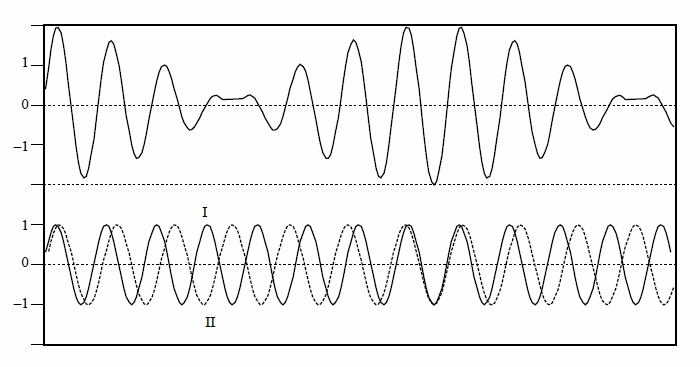
\includegraphics[width=8cm,height=6.4cm]{./02_Capitulos/02_Cap1/figures/fig_06_br.png}
\caption{\label{fig:bestserverarea}- Áreas Preditas de Melhor Servidor de Três Setores.}
\end{center}
\end{figure}

\section{\textbf{Classificação segundo o Método de Cálculo}}
\label{sec:Cap1Metodo}

O primeiro critério de classificação é a maneira pela qual os métodos de localização calculam a estimativa de posição do MS no plano. Para utilizar a geometria euclidiana, é necessário que as coordenadas geográficas dos setores de referência e do MS sejam representadas através uma projeção cartográfica retangular, ou seja, utilizando um sistema de coordenadas cartesianas. Os principais exemplos de sistemas de coordenadas retangulares utilizados em cartografia são o sistema UTM~(\textit{Universal Transverse Mercator})~\cite{Geocartografia}, que utiliza a projeção cartográfica transversa de Mercator, e o sistema MGRS~(\textit{Military Grid Reference System})~\cite{MGRS}.

\subsection{\underline{Identidade da Célula}}
\label{subsec:Cap1Cid}

No método de localização da identidade da célula~(CID - \textit{Cell Identity}), a posição do MS é assumida como sendo igual à da antena transmissora do setor melhor servidor. O método CID, embora seja de baixa complexidade e elevada disponibilidade, apresenta uma precisão muito dependente da densidade de setores na área de interesse~\cite{SPAWC2008}. Assim, o erro de localização pode variar de algumas centenas de metros em áreas urbanas até vários quilômetros em áreas rurais.

\subsection{\underline{Triangulação}}
\label{subsec:Cap1Triangulacao}

As técnicas de triangulação utilizam medidas de distâncias~(multi-lateração) ou ângulos~(multi-angulação) entre o MS e os setores de referência para estimar a localização do MS~\cite{LocationMethodsSurvey2007}.

Todos os métodos de triangulação presumem condições de propagação com linha de visada~(LOS - \textit{Line of Sight}) entre o MS e setores de referência. A propagação por múltiplos percursos e a presença de obstáculos entre o MS e os setores de referência podem corromper as medidas angulares, de tempo e de atenuação no percurso. Assim, a propagação sem linha de visada~(NLOS - \textit{Non Line of Sight}) é a principal fonte de erro para esses métodos. Como a propagação NLOS predomina em ambientes urbanos, a precisão dos métodos de triangulação pode ser seriamente comprometida nesses ambientes.

Além da propagação NLOS, outro fator que limita a precisão dos métodos de triangulação é a resolução finita das medidas realizadas na interface aérea e que são utilizadas no cálculo de posição: tempo, RSS e ângulo de chegada. A resolução da medida de RSS depende de especificações da interface rádio. Em redes GSM e WCDMA, por exemplo, os valores de RSS são reportados pelo MS em passos de $1$ dB~\cite{ETSI100911}~\cite{3GPP25133}. A resolução da medida angular depende da configuração dos conjuntos de antenas diretivas necessários para estimar o ângulo de chegada, bem como do diagrama de irradiação das antenas utilizadas no conjunto~\cite{Rappaport1997}.

\subsubsection{Multi-lateração Circular utilizando RTT}
Um valor de RTT pode ser convertido em uma estimativa de distância, através da equação~(\ref{eq:dist}). O lugar geométrico dos pontos que distam $\hat{d}_{i}$ da $i$-ésima célula de referência é um círculo de raio $\hat{d}_{i}$ centrado na posição desta célula. Esse círculo define o conjunto dos pontos no plano que contém a possível localização do MS, sendo denominado linha de posição (LOP - \textit{Line of Position}).

\begin{equation}
\label{eq:dist}
\hat{d}_{i}= \frac{c \cdot \textrm{T}_{s} \cdot \textrm{RTT}_{i}}{2}
\end{equation}

A medida de RTT tem resolução igual ao período de um símbolo. Porém, por razões de simplificação, utiliza-se a representação por meio de LOPs circulares, com raio igual ao raio interno no anel circular. Quanto menor o período de símbolo, menor é a largura do anel circular e mais este anel aproxima-se de um círculo. Assim, em sistemas banda larga, como o WCDMA, a utilização de LOPs circulares não introduz erro significativo~\cite{CidRttForcedHandover}.

\section{\textbf{Quadro Sinótico}}
\label{sec:Cap1Quadro}

A~\ref{tab:quadrosinotico} resume as principais características dos métodos de localização apresentados neste capítulo: o método de cálculo, a participação do MS no cálculo da posição, a quantidade mínima de setores requerida para calcular a posição do MS e os elementos adicionais necessários na rede de acesso rádio~(RAN - \textit{Radio Access Network}). A última coluna informa se o método depende de condições de propagação LOS entre o MS e as células de referência - ou os satélites, no caso do método AGPS - para não sofrer degradação da acurácia de localização.

Como a precisão de um método de localização é fortemente dependente das características específicas da rede onde o mesmo será utilizado - largura de banda, resolução temporal, densidade superficial de setores, ambiente de propagação, etc. - optou-se por não inserir na~\ref{tab:quadrosinotico} valores genéricos de precisão, como os fornecidos em~\cite{WlanLocationMethodsSurvey}.

\begin{table}[h]
\centering
\caption{\label{tab:quadrosinotico}- Quadro Sinótico dos Métodos de Localização.}
\vspace*{.1cm}
\begin{scriptsize}
\begin{tabular}{|c|c|c|c|c|c|}
\hline
\textbf{Sigla} & \textbf{Método de Cálculo} & \textbf{Participação} & \textbf{Quant. Mín.} & \textbf{Elem. adicionais} & \textbf{Requer}\\
& & \textbf{do MS} & \textbf{de Setores} & \textbf{na RAN} & \textbf{LOS ?}\\
\hline
AOA	& Triang. por multi-angulação & Baseado & 2	& Conj. de antenas & Sim \\
& & na Rede & & diretivas & \\
\hline
CID	& Identidade da célula	& Baseado & 1	& - & Não\\
& & na Rede & & & \\
\hline
EOTD	& Triang. por multi-lateração &	Assistido ou &	3	& LMUs & Sim \\
& hiperbólica & Baseado no MS & & & \\
\hline
AGPS	& Triang. por multi-lateração & Assistido & 3 & - & Sim \\
& circular & pelo MS & & & \\
\hline
CID+RTT	& Triang. por multi-lateração &	Baseado & 3	& - & Sim \\
& circular com RTT & na Rede & & & \\
\hline
CID+RSS	& Triang. por multi-lateração circular  &	Baseado & 3	& - & Sim \\
& com perda de propagação & na Rede & & & \\
\hline
AOA+RTT	& Híbrido	& Baseado & 1	&  Conj. de antenas & Sim \\
& & na Rede & & diretivas & \\
\hline
AOA+RSS	& Híbrido	& Baseado & 1	&  Conj. de antenas & Sim \\
& & na Rede & & diretivas& \\
\hline
AOA+TDOA	& Híbrido	& Assistido & 2	&  Conj. de antenas & Sim \\
& & pelo MS & & diretivas& \\
\hline
\end{tabular}
\end{scriptsize}
\vspace*{-.2cm}
\end{table}


% inserir demais capítulos aqui
% -----------------------------
% -----------------------------
% -----------------------------
% -----------------------------





\pagebreak
\addcontentsline{toc}{chapter}{\hspace{1.7cm}\bfseries CONCLUSÃO}
\noindent\textbf{CONCLUSÃO}
$\!$\\

Aqui entra sua conclusão!!









\pagebreak
\addcontentsline{toc}{chapter}{\hspace{1.7cm}\bfseries REFERÊNCIAS}
\def\bibname{REFERÊNCIAS}



% abaixo segue a chamada para o arquivo [.BIB]. Utilizei o programa JABREF para montar o arquivo com minhas referências.
\bibliography{dissertacao}




%felipe% \printindex    %Removi o índice remissivo para a versão oficial do trabalho.


\end{document}